

\documentclass{article}
\usepackage{CJK}
\usepackage{amsmath,amssymb}
\usepackage{fancyhdr}  
\usepackage{graphicx}
\usepackage{float}

\begin{document}
\begin{CJK*}{GBK}{song}

\pagestyle{fancy}  
\fancyhead{} % clear all fields  
\fancyhead[R]{Data Analysis}  
\fancyhead[L]{Chenxi Gu\\ 2017311017} 
\renewcommand{\headrulewidth}{0.4pt}  
\renewcommand{\footrulewidth}{0.4pt} 



\title {chapter 3}
\author{Chenxi Gu\\2017311017}

\date{\today}

\maketitle

\section{3.1}
\begin{figure}[H]
\centerline{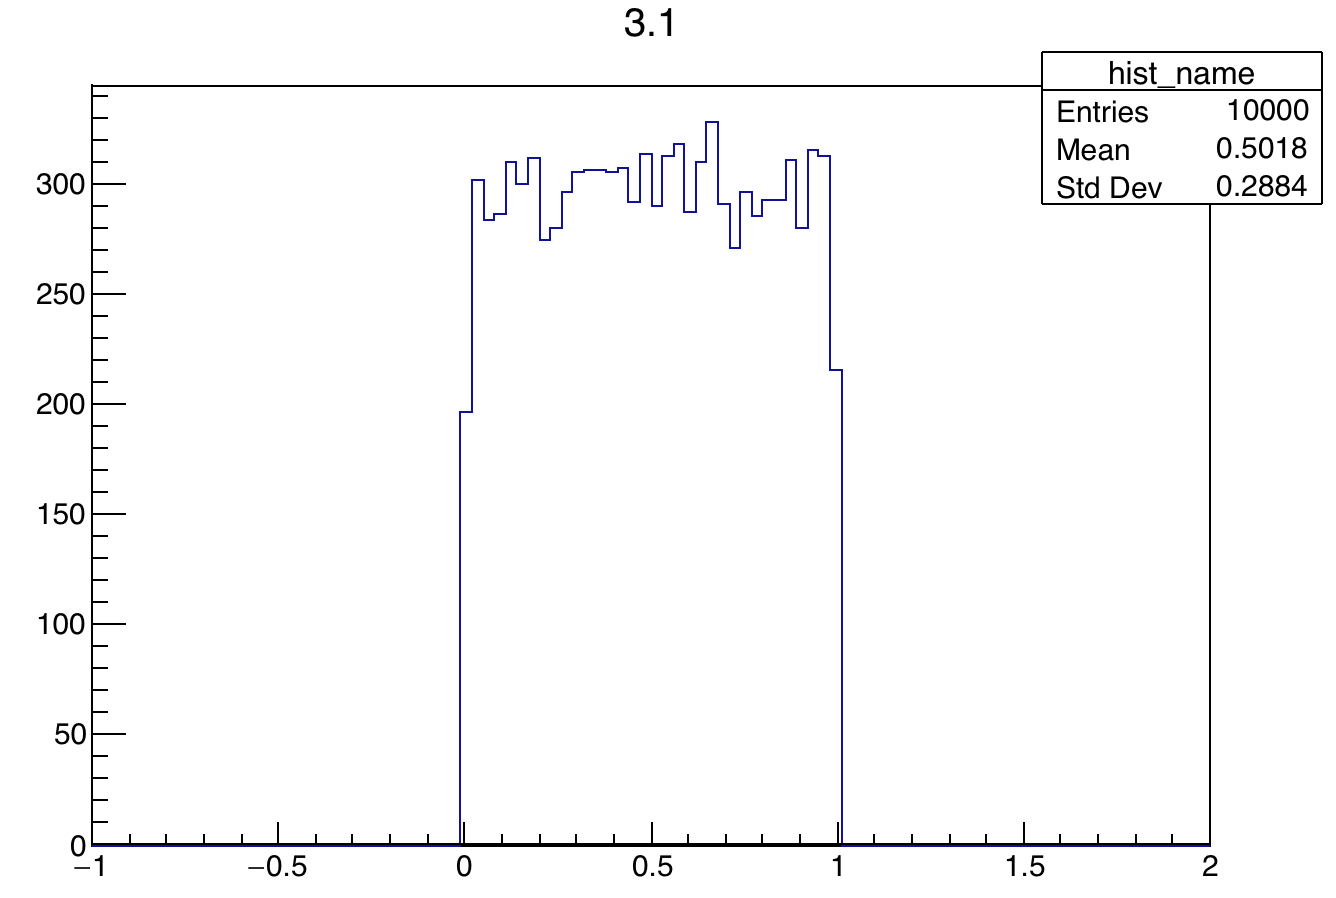
\includegraphics[scale=0.4]{3.1.png}}
\caption{Uniform distribution}
\label{fig:label}
\end{figure}

\section{3.2}
(a)
\begin{figure}[H]
\centerline{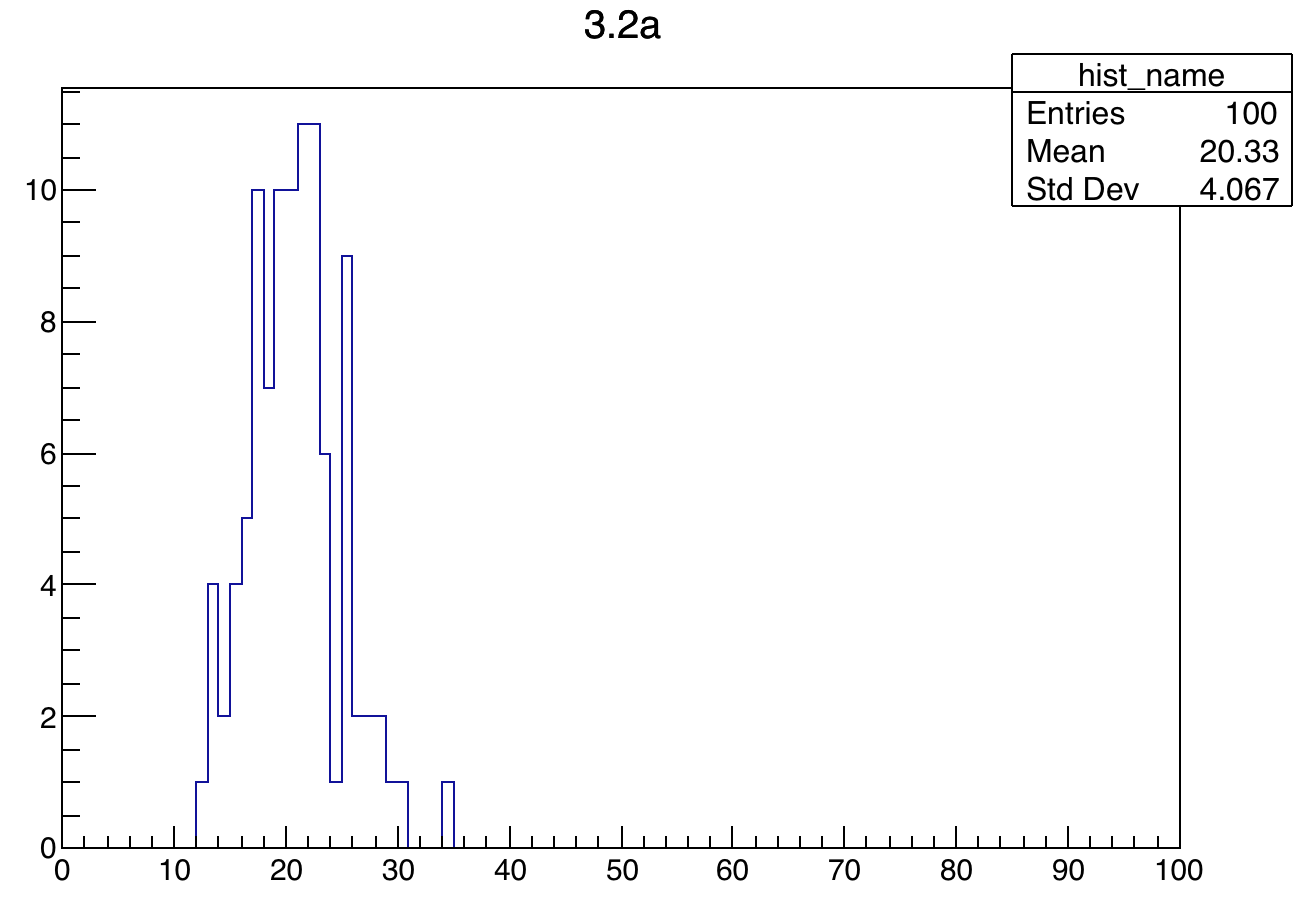
\includegraphics[scale=0.4]{3.2a.png}}
\caption{Binomial distribution}
\label{fig:label}
\end{figure}

(b)
\begin{figure}[H]
\centerline{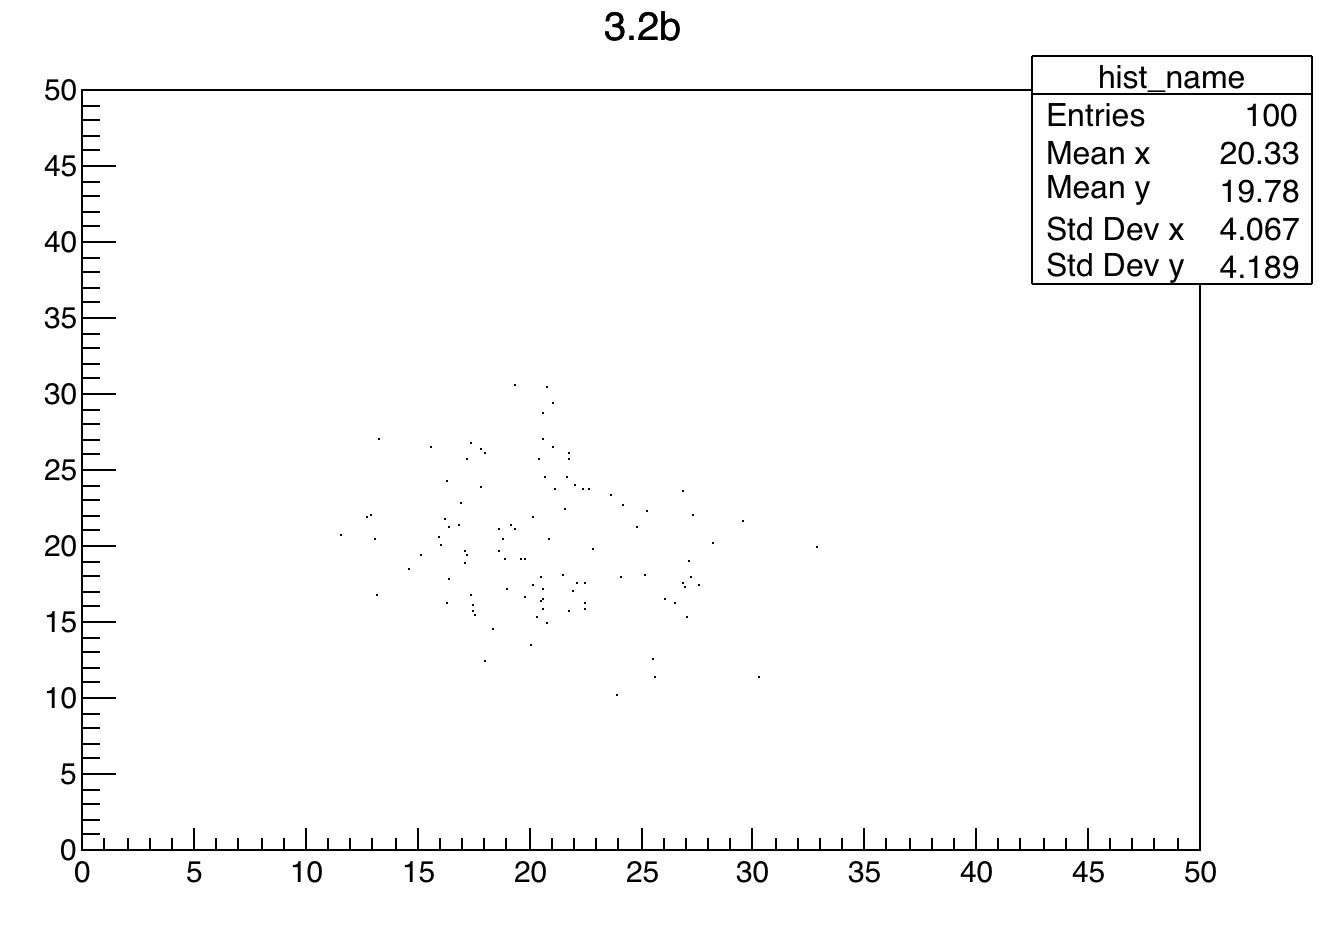
\includegraphics[scale=0.4]{3.2b.png}}
\caption{two dimension histogram}
\label{fig:label}
\end{figure}


\section{3.3}
(a)
\begin{figure}[H]
\centerline{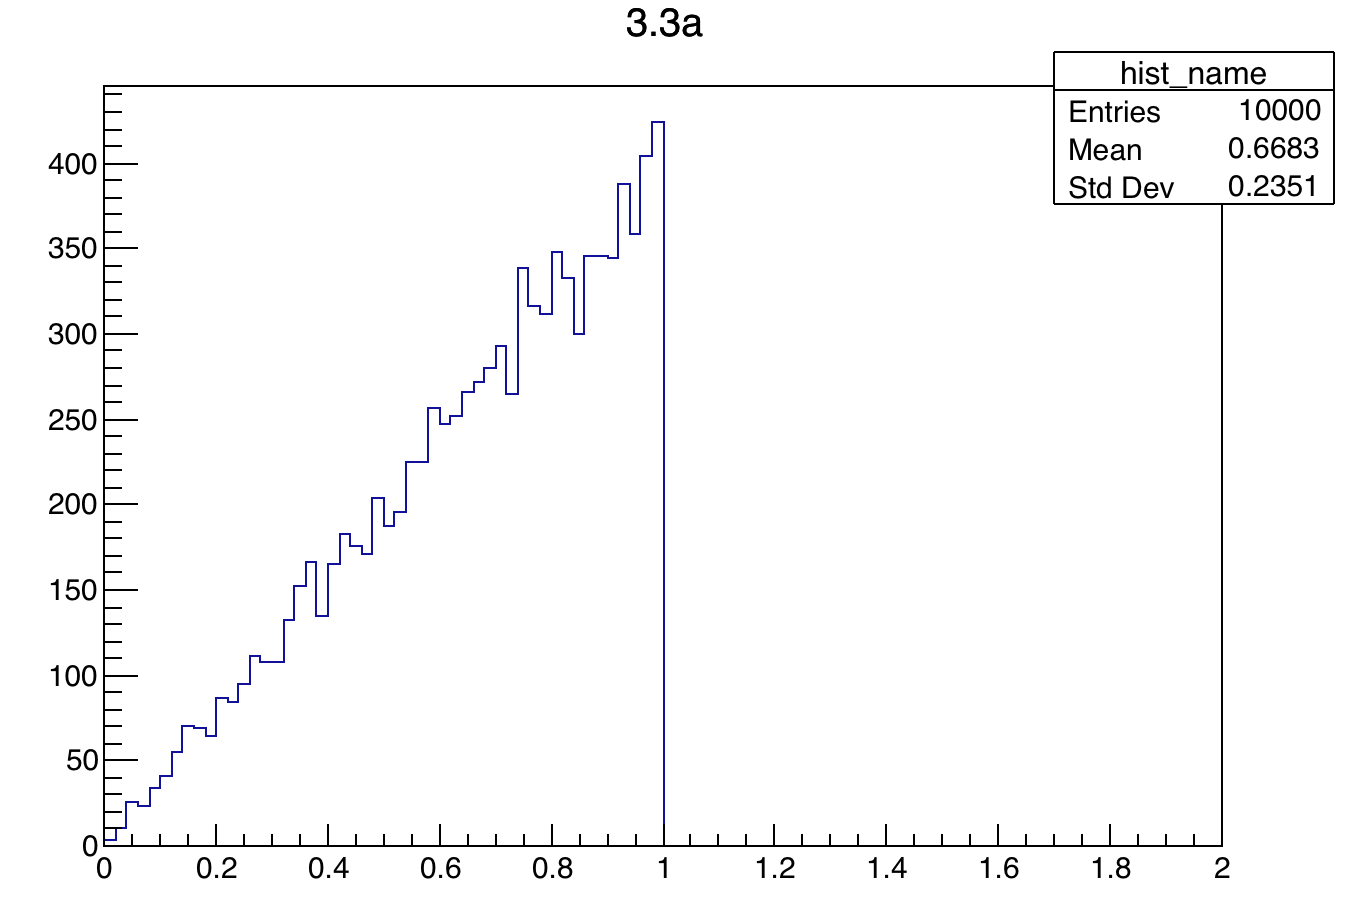
\includegraphics[scale=0.4]{3.3a.png}}
\caption{Histogram}
\label{fig:label}
\end{figure}


(b)
\begin{figure}[H]
\centerline{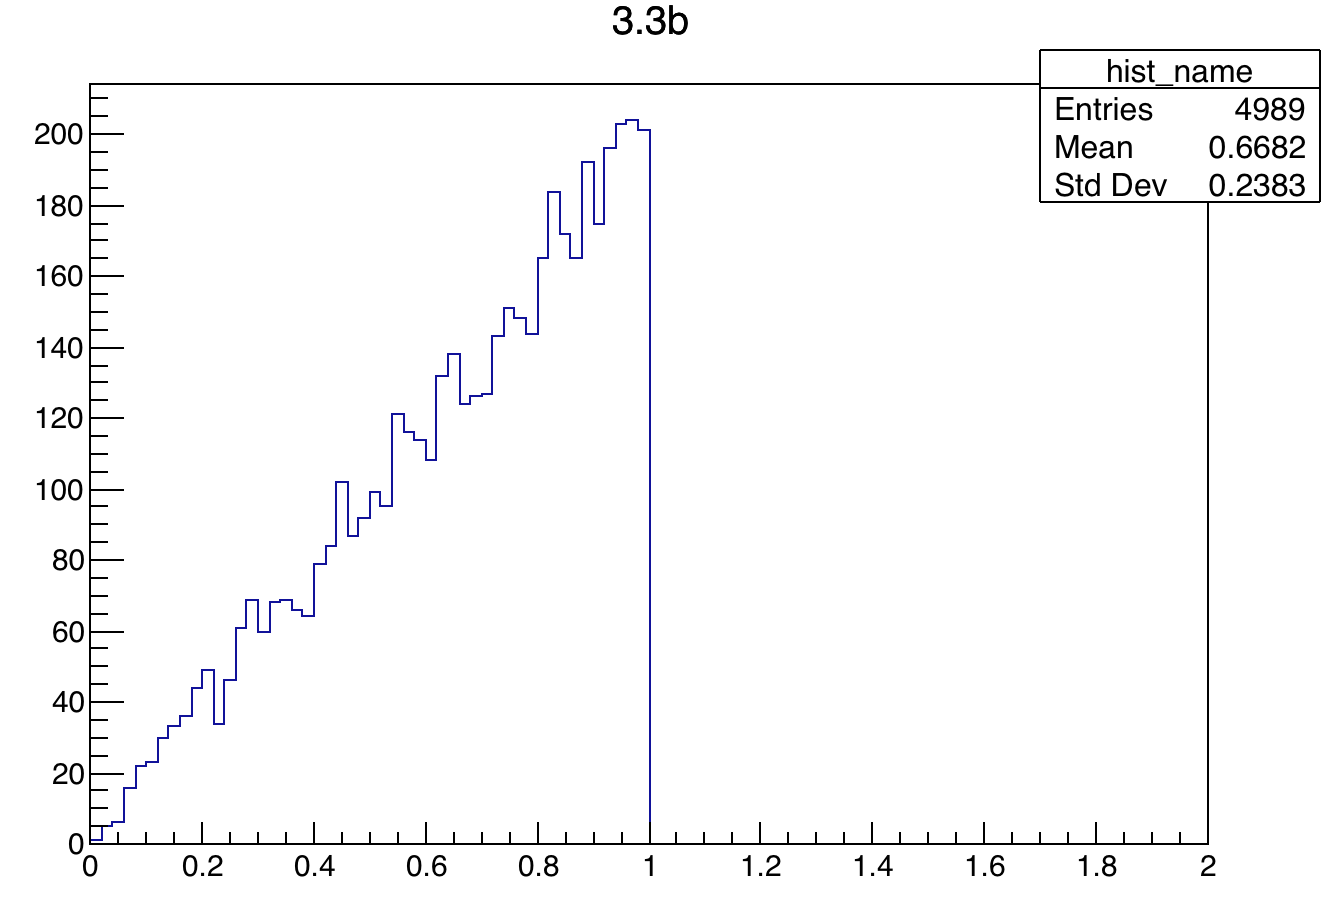
\includegraphics[scale=0.4]{3.3b.png}}
\caption{Histogram}
\label{fig:label}
\end{figure}




\section{3.4}
(a)
\begin{equation}
E(y)=\sum_{i=1}^nE(x_i)=\frac{n}{2}
\end{equation}

\begin{equation}
V(y)=nV(x)=\frac{n}{12}
\end{equation}

\begin{equation}
\begin{aligned}
E(z)&=E\left(\frac{\sum_{i=1}^nx_i-\frac{n}{2}}{\sqrt{n/12}}\right)\\
&=\frac{\sum_{i=1}^nE(x_i)-\frac{n}{2}}{\sqrt{n/12}}\\
&=0
\end{aligned}
\end{equation}
\begin{equation}
V(z)=1
\end{equation}
(b)
\begin{figure}[H]
\centerline{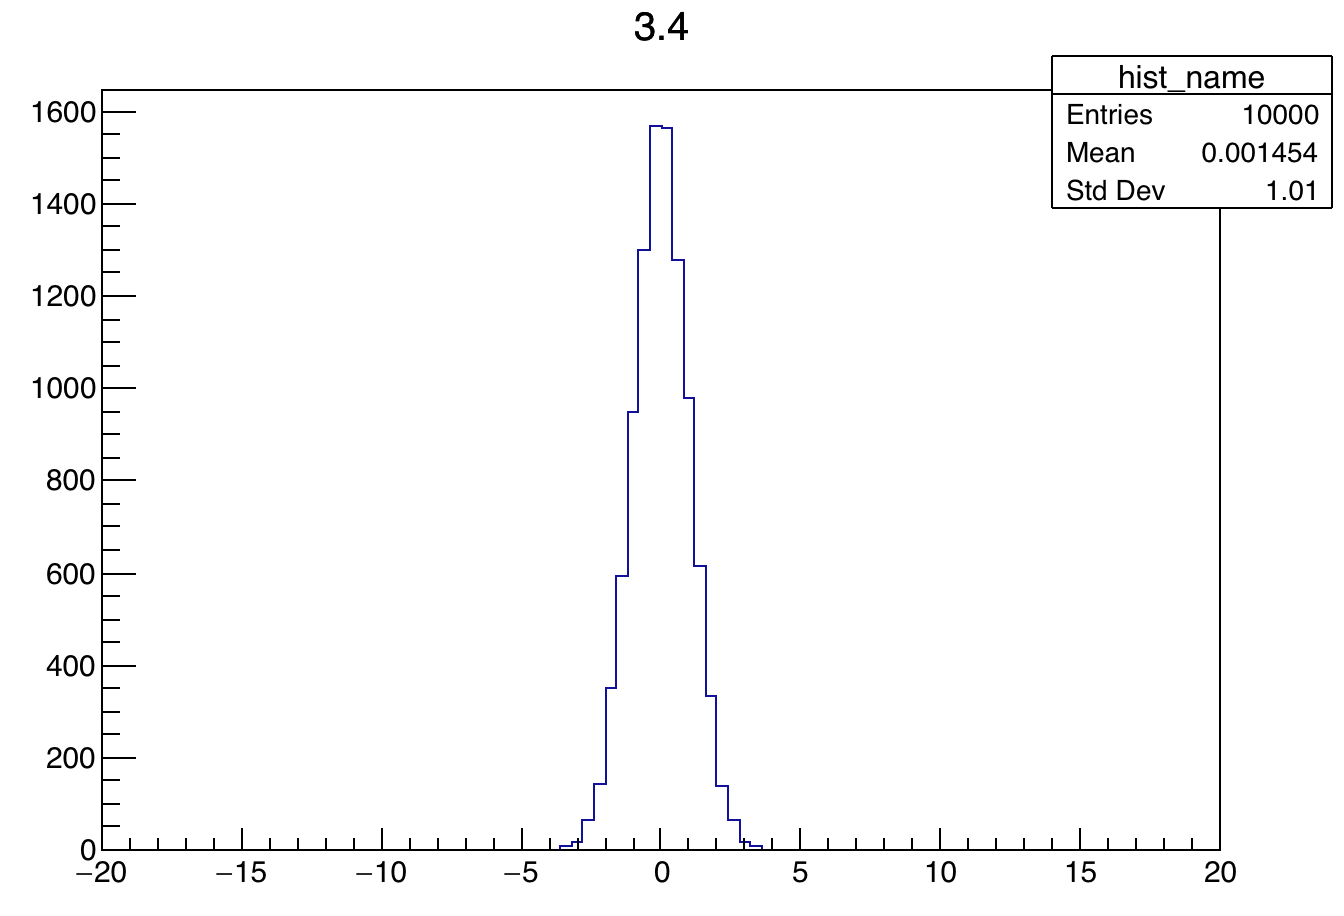
\includegraphics[scale=0.4]{3.4.png}}
\caption{Gaussian distribution}
\label{fig:label}
\end{figure}




\section{3.5}

\begin{figure}[H]
\centerline{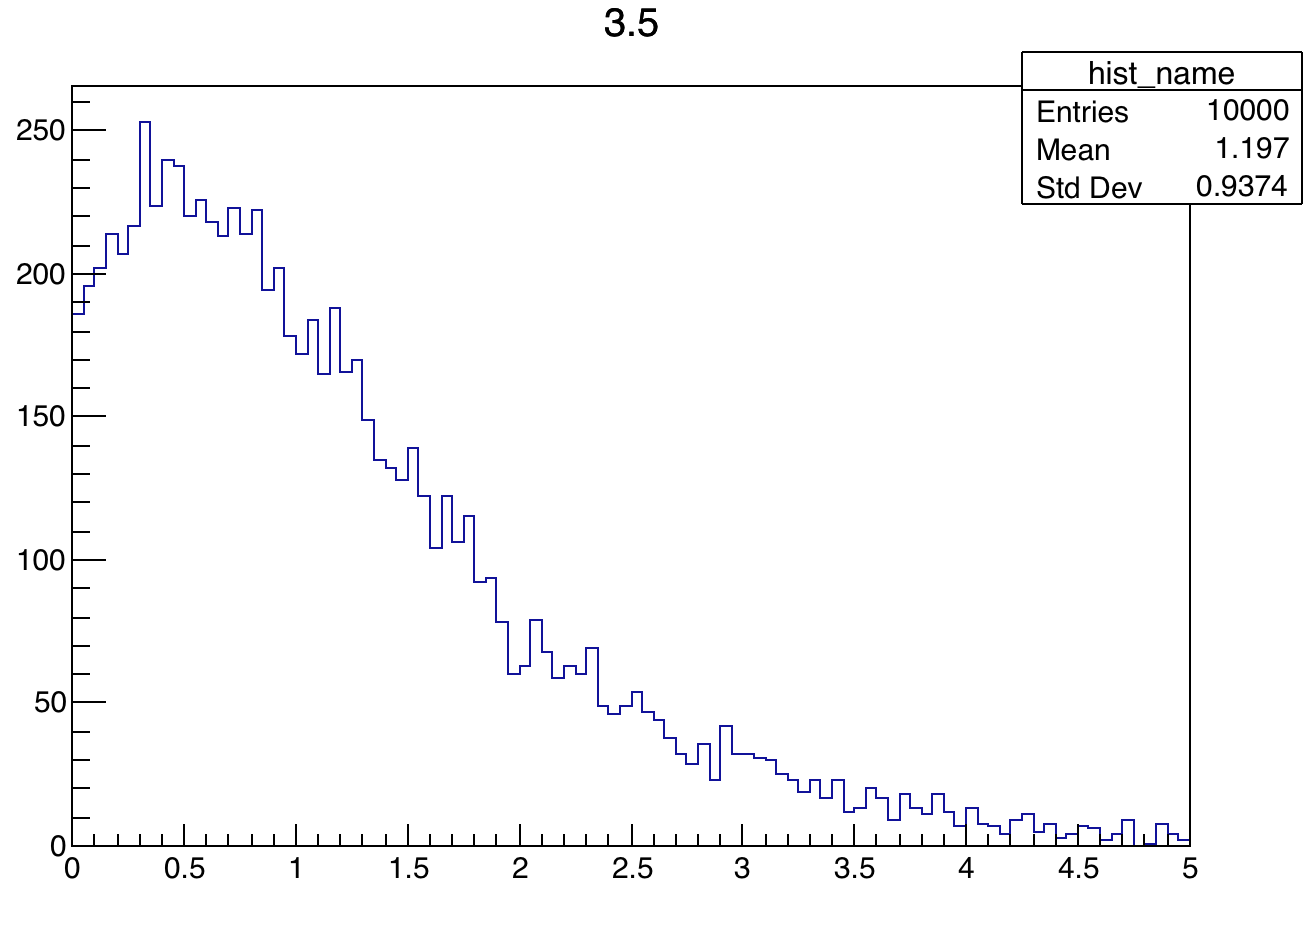
\includegraphics[scale=0.4]{3.5.png}}
\caption{Decay time distribution}
\label{fig:label}
\end{figure}






\section{3.6}
(a)
\begin{equation}
\begin{aligned}
&\int_{-\infty}^{x(r)}f(x)dx=\int_0^rdr=r\\
&\frac{1}{\pi}arctan(x)+\frac{1}{2}=r\\
&x(r)=tan(\pi(r-\frac{1}{2}))
\end{aligned}
\end{equation}

(b)
\begin{figure}[H]
\centerline{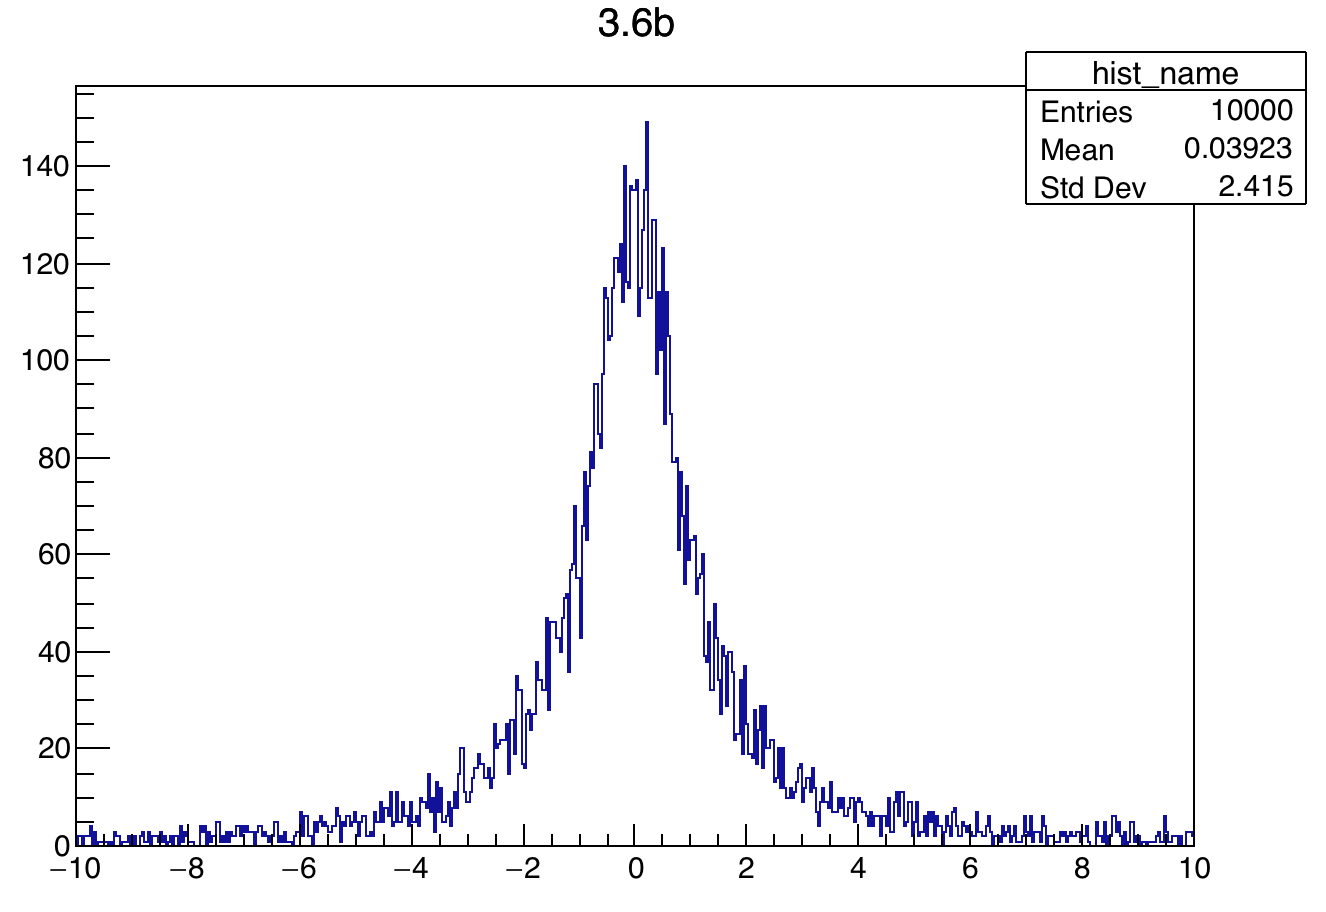
\includegraphics[scale=0.4]{3.6b.png}}
\caption{Cauchy distribution}
\label{fig:label}
\end{figure}

(c)
\begin{figure}[H]
\centerline{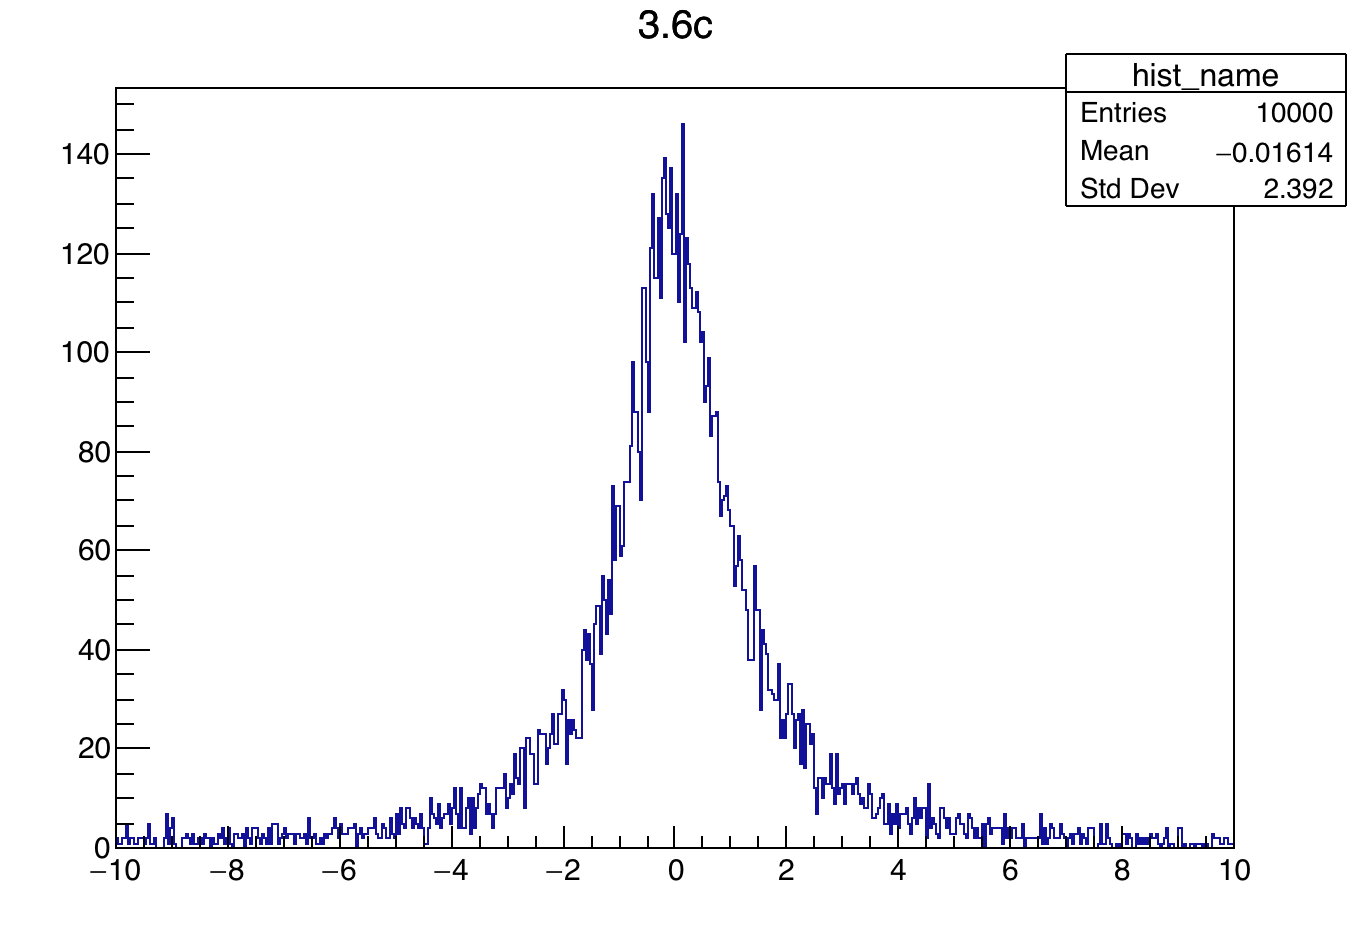
\includegraphics[scale=0.4]{3.6c.png}}
\caption{Cauchy distribution}
\label{fig:label}
\end{figure}







\section{3.7}
(a)
\begin{figure}[H]
\centerline{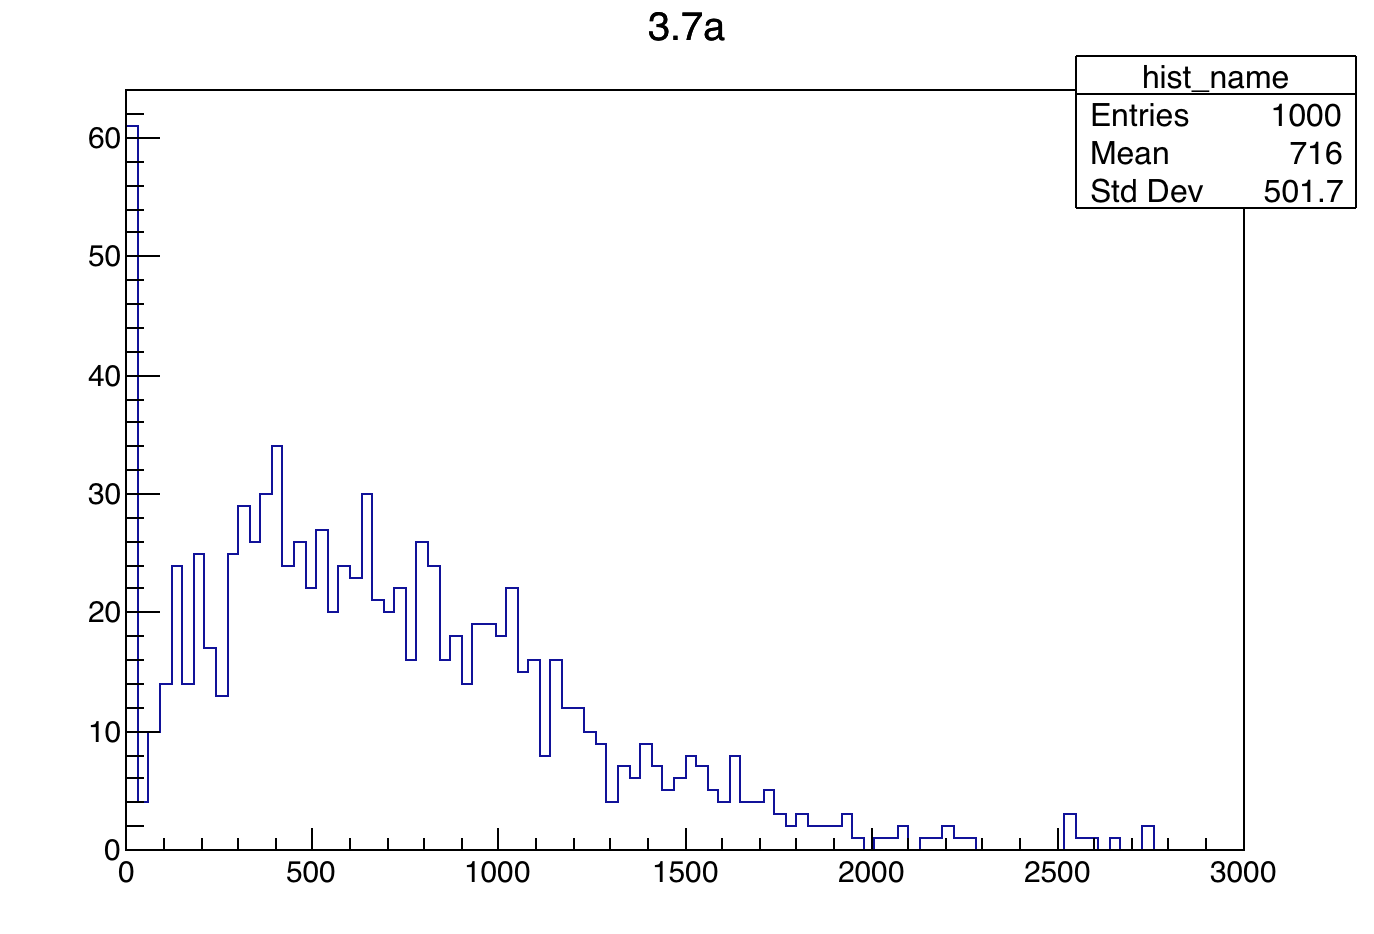
\includegraphics[scale=0.4]{3.7a.png}}
\caption{1000 photon electron distribution}
\label{fig:label}
\end{figure}
the mean value is 716, is very close to the theory mean value 729.\\ 
But the variance is 501.7, the theory variance of the poisson distribution is 729.
\begin{equation}
n_{out}=\prod_{i=1}^6n_{out,i}
\end{equation}
So we should use the Generating Funtions formula:
\begin{equation}
\begin{aligned}
&V^2_{n_{out}}=V^2_{n_{out,1}}+\frac{V^2_{n_{out,2}}}{E(n_{out,1})}+\frac{V^2_{n_{out,3}}}{E(n_{out,1})E(n_{out,2})}....\\
&\sigma_{n_{out}}=\sqrt{364*729}=515
\end{aligned}
\end{equation}
This answer is far away from the poisson distribution which the mean value is 729.\\
(b)
Compare with the figure in (a), $\frac{\sigma_{n_{out}}}{\bar{n}_{out}}$ is smaller. From the formula in (a), We know $V^2_{n_{out,1}}$ is the biggest one in $V^2_{n_{out}}$.
\begin{figure}[H]
\centerline{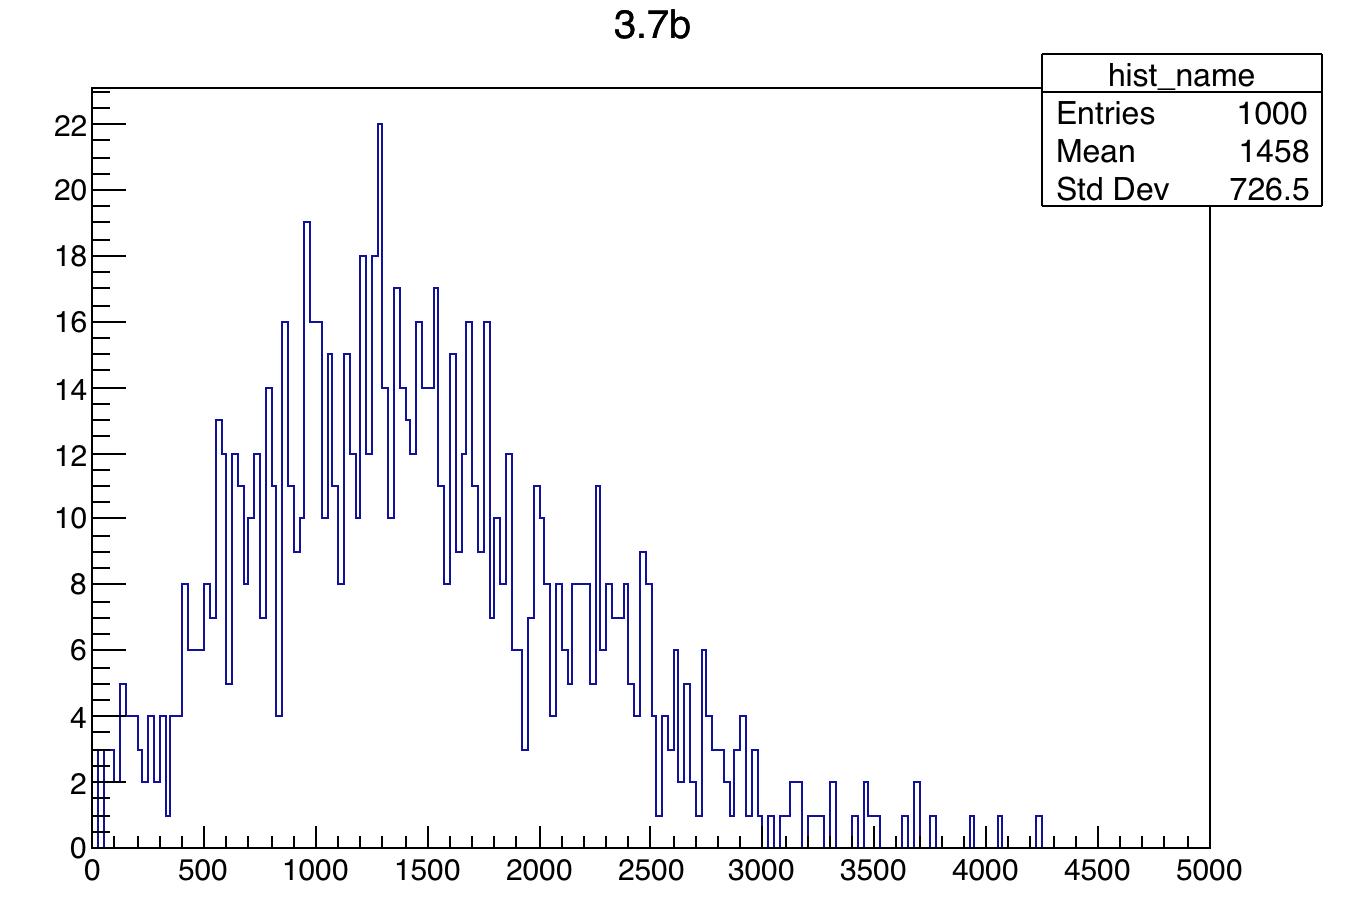
\includegraphics[scale=0.4]{3.7b.png}}
\caption{1000 photon electron distribution}
\label{fig:label}
\end{figure}

(c)
\begin{figure}[H]
\centerline{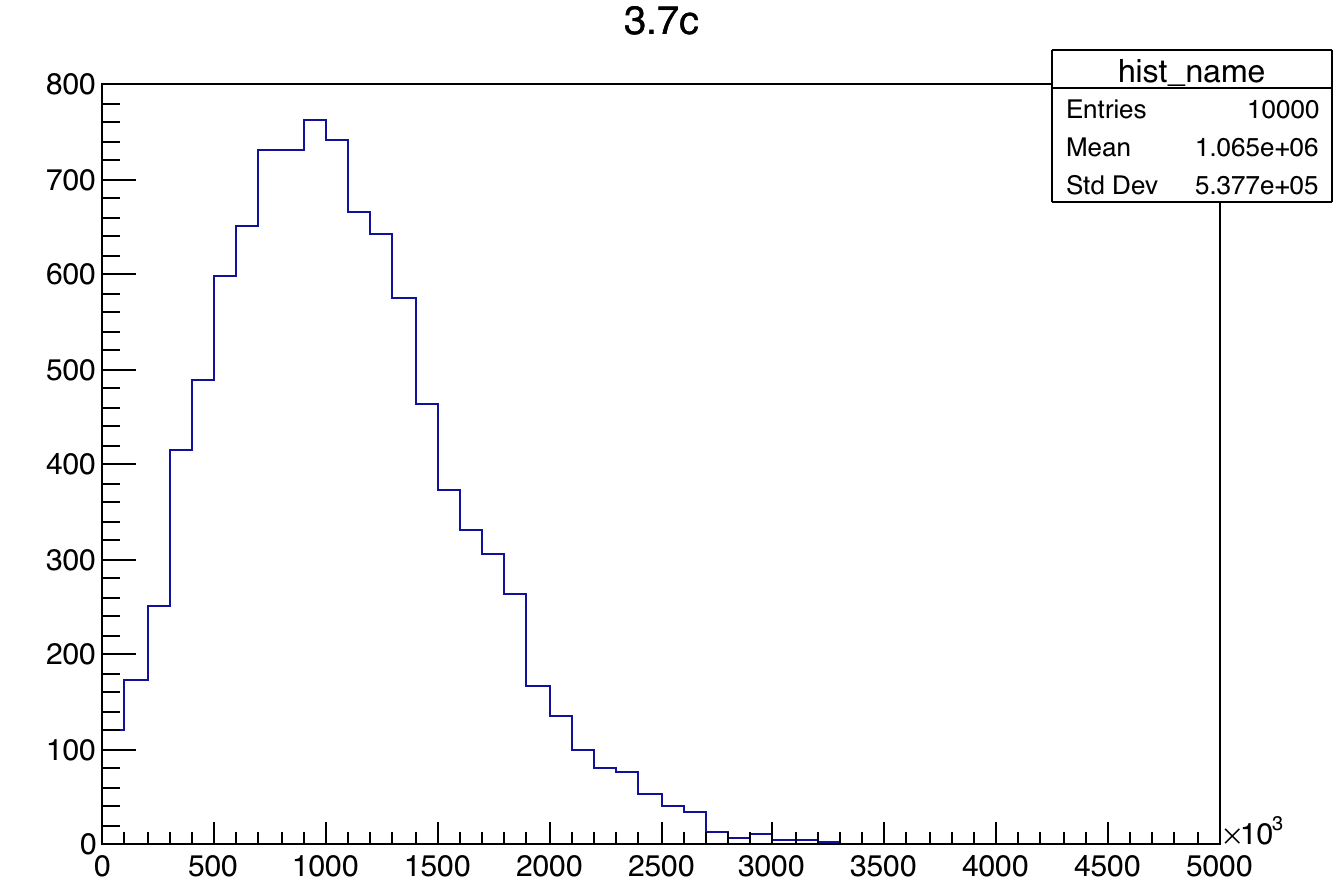
\includegraphics[scale=0.4]{3.7c.png}}
\caption{10000 photon electron distribution}
\label{fig:label}
\end{figure}












\end{CJK*}
\end{document}
